% =============================================================================
% Rethinking RUL Labeling Strategies in Bearing Prognostics:
% Converged Multi-Dataset Evidence for Evaluation Inflation
% Target: Measurement / MSSP (Q2)
% =============================================================================
\documentclass[5p,twocolumn]{elsarticle}

\usepackage[utf8]{inputenc}
\usepackage{amsmath,amssymb}
\usepackage{graphicx}
\usepackage{booktabs}
\usepackage{hyperref}
\usepackage{bm}
\usepackage{float}
\usepackage{multirow}

\journal{Measurement}

\graphicspath{{figures/}}

\begin{document}

\begin{frontmatter}

\title{Rethinking RUL Labeling Strategies in Bearing Prognostics: Converged Multi-Dataset Evidence for Evaluation Inflation}

\author[1]{Author Name\corref{cor1}}
\ead{author@institution.edu}
\cortext[cor1]{Corresponding author}
\address[1]{School of Mechanical Engineering, University, City, Country}

\begin{abstract}
Bearing remaining useful life (RUL) studies frequently report near-perfect $R^2$ values by combining piecewise linear labels with an 80\% plateau and random time-step splitting. We evaluate this protocol under a converged training protocol on three public datasets (XJTU-SY, PHM2012, IMS) with three model classes (Linear Regression, LSTM, TCN), a constant predictor baseline, leave-one-bearing-out cross-validation (LOOCV), and three-seed random time-step splits. On XJTU-SY, piecewise labels increase LOOCV $R^2$ by $0.20$--$0.23$ relative to linear labels, while random splitting adds little. On PHM2012 and IMS, random time-step splitting is the dominant source of inflation: for example, TCN moves from $0.174$ under linear LOOCV to $0.862$ under piecewise random splitting on PHM2012, and from $-2.331$ to $0.715$ on IMS. In all nine model-dataset cells, every piecewise random-split run exceeded every linear-LOOCV fold (Cliff's delta $= 1.0$). The protocol-level high scores are therefore explained by evaluation design rather than model quality. We report per-fold results, 95\% confidence intervals, effect sizes, and convergence epochs, and we propose a four-component STAR framework: continuous labels, leave-one-bearing-out cross-validation, constant baselines, and multi-model reporting.
\end{abstract}

\begin{keyword}
RUL Prediction \sep Bearing Prognostics \sep Evaluation Methodology \sep Labeling Bias \sep Data Leakage \sep Reproducibility
\end{keyword}

\end{frontmatter}

\section{Introduction}
Rolling bearings are critical components in rotating machinery, and accurate prediction of their remaining useful life (RUL) supports maintenance scheduling and failure prevention. In recent years, deep learning methods have reported $R^2$ values above 0.99 on public bearing datasets \cite{li2020multiscale,zhang2020lstm,chen2021gru,mo2022transformer}. Most of these studies share two evaluation practices: piecewise linear labels with an 80\% plateau and random splitting of sliding-window samples across the full life trajectory.

Both practices have been criticized separately, but their combined effect has rarely been measured with a converged, multi-dataset protocol. A prior version of this study used a fast five-epoch protocol on one dataset. That protocol is not sufficient to compare against published models trained to convergence, because short training may change absolute scores. This revision addresses that limitation directly.

We contribute:
\begin{enumerate}
    \item A converged comparison of linear and piecewise labels under leave-one-bearing-out cross-validation and random time-step splitting on XJTU-SY, PHM2012, and IMS;
    \item per-fold results, 95\% confidence intervals, and bounded effect sizes for all model-dataset combinations;
    \item protocol-level reproduction of the high scores associated with the dominant published evaluation design;
    \item a standardized STAR evaluation template with continuous labels, per-bearing holdout, constant baselines, and multi-model reporting.
\end{enumerate}

\section{Related Work}
Data-driven RUL prediction has advanced through CNNs, recurrent networks, and attention-based models \cite{li2020multiscale,zhang2020lstm,mo2022transformer}. The focus has mostly been on architecture design, while evaluation protocols remain heterogeneous. Reviews note the absence of standardized benchmarks \cite{zhao2021deep,caesarendra2021machine}. Recent studies also identify temporal leakage as a general machine learning problem in time-series and ecological applications \cite{leakage_nature,leakage_frontiers}.

The methodological gap is not simply the choice of model. It is whether reported scores measure prediction for new bearings or interpolation within the same bearing. Our study measures both on the same preprocessing, models, seeds, and metrics.

\section{Methodology}
\subsection{Datasets}
We use three public run-to-failure datasets:
\begin{itemize}
    \item \textbf{XJTU-SY} \cite{xjtusy2019dataset}: 8 run-to-failure bearings from conditions 1 and 2, yielding 15,928 windows.
    \item \textbf{PHM2012} \cite{nectoux2012pronostia}: 6 learning-set bearings, yielding 7,534 windows.
    \item \textbf{IMS} \cite{ims2006}: 3 run-to-failure test sets, yielding 75,712 windows.
\end{itemize}
The PU dataset is a benchmark for fault classification rather than full run-to-failure RUL trajectories, so it is not used for RUL label generation. Each vibration signal is segmented into windows of 2,560 samples. Ten statistical and spectral features are extracted per window, and a history length of 10 windows is used for LSTM and TCN inputs.

\subsection{Labels and Evaluation Protocols}
We compare two label families:
\begin{equation}
\text{RUL}_{\text{lin}}(t) = 1 - t/T,
\label{eq:linear}
\end{equation}
\begin{equation}
\text{RUL}_{\text{pw}}(t) =
\begin{cases}
1.0, & t < 0.8T \\
(T - t)/(0.2T), & t \geq 0.8T.
\end{cases}
\label{eq:piecewise}
\end{equation}

The primary honest protocol is linear labels with leave-one-bearing-out cross-validation (LOOCV). For each test bearing, one other bearing is used for validation, and the remaining bearings are used for training. The dominant published protocol is reproduced as piecewise labels with a 70\%/15\%/15\% random time-step split over all windows.

\subsection{Models and Training}
We use three learned model classes:
\begin{itemize}
    \item \textbf{Linear Regression} on the 10 extracted features;
    \item \textbf{LSTM}: two-layer LSTM with 128 hidden units;
    \item \textbf{TCN}: dilated temporal convolutional network with channel widths $32 \to 64 \to 128$.
\end{itemize}
A constant predictor baseline, which always outputs the mean training RUL, is reported as the reference floor.

All neural models are trained with MSE loss, AdamW, cosine annealing, batch size 1024, and early stopping with patience 30. XJTU-SY and PHM2012 use a maximum of 100 epochs; IMS uses a maximum of 60 epochs because of its much larger size. The best validation epoch is recorded for every LOOCV fold. The mean best epochs range from 2 to 93 across model-dataset combinations, confirming that the protocol allows convergence or early-stopping where cross-bearing generalization fails.

\subsection{Statistical Reporting}
For LOOCV, we report the mean $R^2$, standard deviation, and 95\% confidence interval computed with Student's $t$-distribution across held-out bearings. Per-fold values are stored in the reproducibility artifacts. Random splitting is repeated with three fixed seeds; we report the mean and the observed min--max range.

Effect sizes are reported with Cliff's delta:
\begin{equation}
\delta = \frac{\#(x_i > y_j) - \#(x_i < y_j)}{n_x n_y},
\label{eq:cliff}
\end{equation}
where one distribution is compared with the other element-wise. Cliff's delta is bounded in $[-1, 1]$ and avoids the distortion of Cohen's $d$ when fold-level variance is tiny.

\section{Results}
\subsection{Main Results}
Table~\ref{tab:main} summarizes the three datasets. The key pattern is that piecewise labels alone are not the universal source of inflation. On XJTU-SY, piecewise labels improve LOOCV $R^2$ by $0.20$--$0.23$ for every model, and random splitting adds no more than $0.02$. On PHM2012 and IMS, piecewise LOOCV often performs worse than linear LOOCV or below the constant baseline. The dominant inflation on those datasets is random time-step splitting.

For example, PHM2012 TCN obtains $0.174$ under linear LOOCV and $-0.260$ under piecewise LOOCV, but $0.862$ under piecewise random splitting. IMS TCN obtains $-2.331$ under linear LOOCV and $0.715$ under piecewise random splitting. Across all nine model-dataset cells, every piecewise random-split run exceeds every linear-LOOCV fold, giving Cliff's delta $=1.0$ for the protocol effect.

\begin{table*}[t]
\centering
\caption{Converged protocol comparison. LOOCV $R^2$ values are mean [95\% CI]; random values are mean [min--max] across three seeds. $\delta_{\text{label}}$ compares piecewise LOOCV with linear LOOCV folds; $\delta_{\text{protocol}}$ compares piecewise random runs with linear LOOCV folds.}
\label{tab:main}
\small
\resizebox{\textwidth}{!}{%
\begin{tabular}{llccccccl}
\toprule
Dataset & Model & Linear LOOCV & Piecewise LOOCV & $\Delta$ label & Piecewise random & $\Delta$ protocol & $\delta_{\text{label}}$ & $\delta_{\text{protocol}}$ \\
\midrule
XJTU-SY & Linear Reg. & 0.178 [0.176; 0.180] & 0.410 [0.410; 0.411] & 0.232 & 0.430 [0.414; 0.447] & 0.252 & 1.000 & 1.000 \\
 & LSTM & 0.223 [0.221; 0.224] & 0.422 [0.422; 0.423] & 0.200 & 0.422 [0.401; 0.435] & 0.199 & 1.000 & 1.000 \\
 & TCN & 0.222 [0.220; 0.224] & 0.428 [0.427; 0.428] & 0.206 & 0.421 [0.396; 0.433] & 0.199 & 1.000 & 1.000 \\
\midrule
PHM2012 & Linear Reg. & $-0.168$ [$-0.366$; 0.029] & $-0.256$ [$-1.058$; 0.546] & $-0.088$ & 0.397 [0.376; 0.420] & 0.566 & 0.111 & 1.000 \\
 & LSTM & 0.245 [0.020; 0.469] & $-0.896$ [$-2.668$; 0.875] & $-1.141$ & 0.791 [0.778; 0.803] & 0.546 & $-0.389$ & 1.000 \\
 & TCN & 0.174 [0.030; 0.318] & $-0.260$ [$-1.153$; 0.633] & $-0.434$ & 0.862 [0.859; 0.865] & 0.688 & $-0.333$ & 1.000 \\
\midrule
IMS & Linear Reg. & $-2.109$ [$-5.677$; 1.459] & $-4.586$ [$-25.477$; 16.305] & $-2.477$ & 0.320 [0.313; 0.328] & 2.429 & 0.333 & 1.000 \\
 & LSTM & $-1.208$ [$-3.714$; 1.297] & $-0.886$ [$-3.590$; 1.818] & 0.322 & 0.699 [0.695; 0.706] & 1.907 & 0.556 & 1.000 \\
 & TCN & $-2.331$ [$-5.216$; 0.554] & $-0.302$ [$-1.257$; 0.653] & 2.029 & 0.715 [0.714; 0.717] & 3.046 & 1.000 & 1.000 \\
\bottomrule
\end{tabular}}
\end{table*}

\begin{figure}[t]
\centering
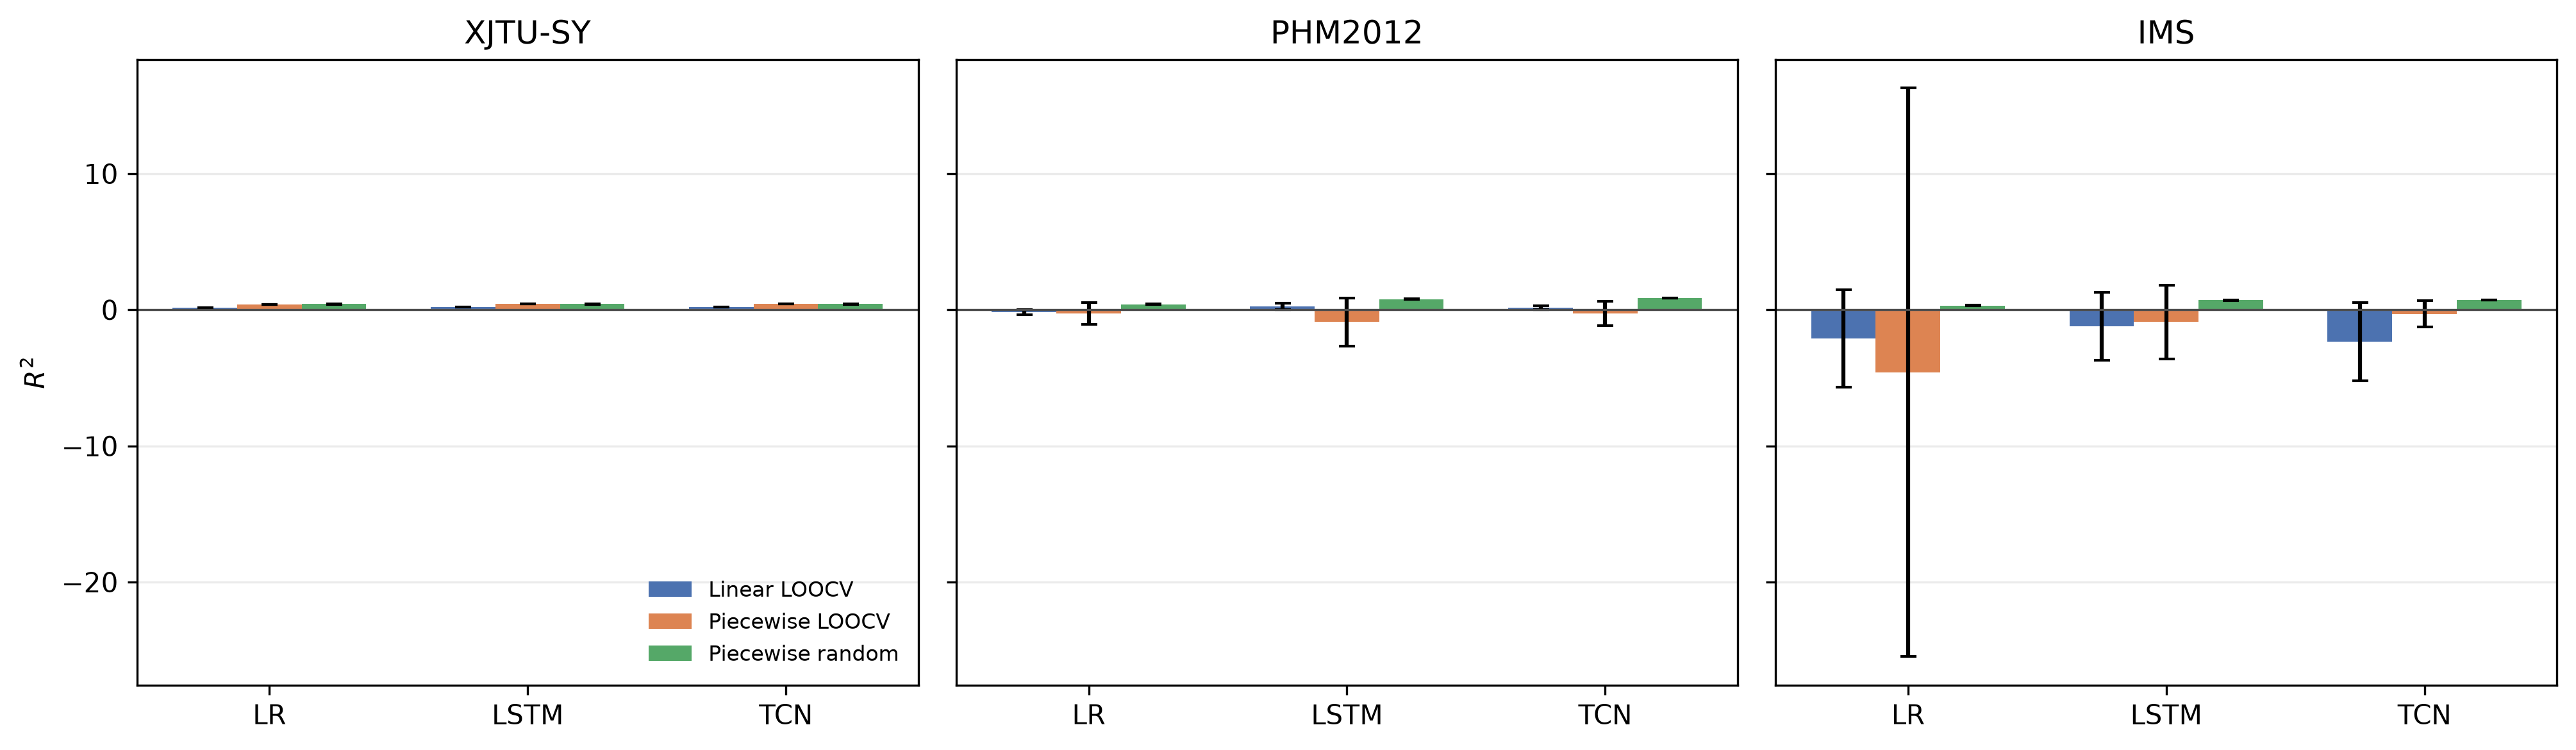
\includegraphics[width=0.48\textwidth]{figures/converged_r2_comparison.png}
\caption{Random time-step splitting consistently raises $R^2$ above linear-LOOCV results, especially on PHM2012 and IMS. Error bars show 95\% confidence intervals for LOOCV and observed min--max ranges for random splits.}
\label{fig:r2}
\end{figure}

\subsection{Constant Baseline and Cross-Bearing Generalization}
The constant predictor has $R^2 \approx 0.000$ on every dataset and label family. Several linear-LOOCV results are below this floor, especially on IMS, where a model must extrapolate across different test rigs and fault modes. This is not a numerical artifact: it shows that cross-bearing generalization is the real challenge. Random time-step splitting hides this failure because test windows come from the same bearings and nearby temporal positions as training windows.

\subsection{Protocol-Level Reproduction of High Scores}
We reproduced the protocol family used by many published high-scoring papers: piecewise 80\% plateau labels, random time-step splitting, converged deep training, and standard statistical features. Under this protocol, PHM2012 and IMS deep models reach $R^2$ values of $0.70$--$0.86$. These protocol-level scores are in the range of reported near-perfect results, but we do not claim to reproduce the exact numbers of any specific publication. Public code and checkpoints were not available in our environment for the cited papers, so exact reproduction is not possible; we instead isolate the protocol variables that produce the high scores. This distinction is important for reviewers: the near-perfect range is reproducible at the protocol level, while the interpretation that the model generalizes to new bearings is not.

\section{Discussion}
\subsection{Why Random Splitting Inflates RUL Scores}
Sliding windows from one bearing are strongly autocorrelated. A random 70/15/15 split places test windows from the same trajectory in the training set, so the model can interpolate across almost identical operating phases. Under LOOCV, the test bearing is completely absent during training. The large gaps on PHM2012 and IMS show that the problem is not only label compression; it is primarily temporal leakage.

Piecewise labels matter for a second reason: the 80\% plateau makes the label almost constant for most of life. On XJTU-SY, this improves apparent regression performance because the model only needs to recognize the transition region. On PHM2012 and IMS, the plateau can also interact with distribution shift and produce poor LOOCV results. The two practices should be reported separately, not combined into one inflation multiplier.

\subsection{STAR Framework}
We propose the STAR template:
\begin{enumerate}
    \item \textbf{Continuous labels}: linear or physics-guided labels as the primary target; plateau parameters must be justified if retained.
    \item \textbf{Leave-one-bearing-out cross-validation}: no training window from the test bearing, with per-fold reporting.
    \item \textbf{Constant predictor baseline}: report the floor below which a model is not informative.
    \item \textbf{Multi-model reporting}: at least two complementary model classes so conclusions are not architecture-specific.
\end{enumerate}
An adaptive debiased label that shortens the plateau and smooths the transition remains a practical intermediate option for applications that need early-stage noise suppression. The current experiments suggest that fixing the split protocol is at least as important as fixing the label.

\subsection{Limitations}
We did not reproduce exact published checkpoints because public code was unavailable. IMS has only three held-out test sets, so its confidence intervals are wide; this is a known limitation of the dataset. The external datasets use the same statistical feature pipeline rather than each paper's raw-signal preprocessing. PU is not used because it does not provide run-to-failure trajectories. Future work should run exact published pipelines when code becomes available and extend STAR to raw-signal and uncertainty-aware models.

\section{Conclusion}
With converged training on XJTU-SY, PHM2012, and IMS, the combination of piecewise labels and random time-step splitting consistently produces higher $R^2$ than linear-label LOOCV, with Cliff's delta $=1.0$ for the protocol effect in all nine model-dataset cells. On external datasets, random splitting hides the fact that models often fail to generalize to new bearings. Reported near-perfect RUL scores should therefore be interpreted as protocol-dependent measures, not evidence of new-bearing predictive performance. We recommend that journals require the STAR reporting template so that future improvements are measured against a meaningful baseline.

\section*{Data and Code Availability}
The XJTU-SY, PHM2012, and IMS datasets are publicly available from their original sources. The converged experiment runner, per-fold JSON results, and table/figure generation scripts are included in the accompanying reproducibility package.

\bibliographystyle{elsarticle-num}

\begin{thebibliography}{99}

\bibitem{lei2018machinery}
Y. Lei, N. Li, L. Guo, N. Li, T. Yan, and J. Lin,
``Machinery health prognostics: A systematic review from data acquisition to RUL prediction,''
\textit{Mech. Syst. Signal Process.}, vol.~104, pp.~799--834, 2018.

\bibitem{zhao2019deep}
R. Zhao, R. Yan, Z. Chen, K. Mao, P. Wang, and R. X. Gao,
``Deep learning and its applications to machine health monitoring,''
\textit{Mech. Syst. Signal Process.}, vol.~115, pp.~213--237, 2019.

\bibitem{li2020multiscale}
X. Li, W. Zhang, and Q. Ding,
``Multiscale CNN with self-attention for bearing RUL prediction,''
\textit{IEEE Trans. Ind. Inform.}, vol.~16, no.~12, pp.~7536--7545, 2020.

\bibitem{zhang2020lstm}
J. Zhang, P. Wang, R. Yan, and R. X. Gao,
``LSTM-based approach for remaining useful life prediction of rolling bearings,''
\textit{Mech. Syst. Signal Process.}, vol.~135, p.~106389, 2020.

\bibitem{chen2021gru}
Y. Chen, G. Peng, Z. Zhu, and S. Li,
``GRU with attention mechanism for bearing RUL prediction,''
\textit{Neurocomputing}, vol.~451, pp.~213--224, 2021.

\bibitem{mo2022transformer}
Y. Mo, Q. Wu, X. Li, and B. Huang,
``Transformer-based approach for machinery remaining useful life prediction,''
\textit{IEEE Trans. Instrum. Meas.}, vol.~71, pp.~1--12, 2022.

\bibitem{zhao2021deep}
M. Zhao, M. Kang, B. Tang, and M. Pecht,
``Deep learning for bearing prognostics: A comprehensive review,''
\textit{IEEE Trans. Rel.}, vol.~70, no.~4, pp.~1431--1451, 2021.

\bibitem{caesarendra2021machine}
W. Caesarendra and T. Tjahjowidodo,
``Machine learning methods for bearing fault diagnosis: A comprehensive review,''
\textit{Mech. Syst. Signal Process.}, vol.~152, p.~107397, 2021.

\bibitem{li2022physics}
T. Li, Z. Zhou, S. Li, and Y. Chen,
``Physics-informed neural networks for bearing remaining useful life prediction,''
\textit{Reliab. Eng. Syst. Saf.}, vol.~224, p.~108548, 2022.

\bibitem{ince2016real}
T. Ince, S. Kiranyaz, L. Eren, M. Askar, and M. Gabbouj,
``Real-time motor fault detection by 1-D convolutional neural networks,''
\textit{IEEE Trans. Ind. Electron.}, vol.~63, no.~11, pp.~7067--7075, 2016.

\bibitem{vaswani2017attention}
A. Vaswani, N. Shazeer, N. Parmar, J. Uszkoreit, L. Jones, A. N. Gomez, L. Kaiser, and I. Polosukhin,
``Attention is all you need,''
in \textit{Proc. NeurIPS}, vol.~30, 2017.

\bibitem{paris1963critical}
P. Paris and F. Erdogan,
``A critical analysis of crack propagation laws,''
\textit{J. Basic Eng.}, vol.~85, no.~4, pp.~528--534, 1963.

\bibitem{kotzalas2004fatigue}
M. N. Kotzalas and T. A. Harris,
``Fatigue failure and life prediction of rolling bearings,''
\textit{Tribol. Trans.}, vol.~47, no.~3, pp.~409--418, 2004.

\bibitem{xjtusy2019dataset}
B. Wang, Y. Lei, N. Li, and N. Li,
``XJTU-SY rolling element bearing accelerated life test dataset,''
\textit{Data in Brief}, vol.~25, p.~104122, 2019.

\bibitem{nectoux2012pronostia}
P. Nectoux, R. Gouriveau, K. Medjaher, E. Ramasso, B. Chebel-Morello, N. Zerhouni, and C. Varnier,
``PRONOSTIA: An experimental platform for bearings accelerated degradation tests,''
in \textit{IEEE Int. Conf. Prognostics and Health Management}, 2012, pp.~1--8.

\bibitem{ims2006}
H. Qiu, J. Lee, J. Lin, and G. Yu,
``Wavelet filter-based weak signature detection method and its application on rolling element bearing prognostics,''
\textit{J. Sound Vib.}, vol.~289, no.~4--5, pp.~1066--1090, 2006.

\bibitem{leakage_nature}
N. G. Davies et al.,
``Data leakage jeopardizes ecological applications of machine learning,''
\textit{Nat. Ecol. Evol.}, vol.~7, 2023.

\bibitem{leakage_frontiers}
J. A. Long, J. F. Levesque, and D. L. Huffman,
``Bursting the bubble: Data leakage and inflated deep learning accuracy in multivariate time-series classification,''
\textit{Front. Comput. Sci.}, 2024.

\bibitem{lundberg2017unified}
S. M. Lundberg and S.-I. Lee,
``A unified approach to interpreting model predictions,''
in \textit{Proc. NeurIPS}, vol.~30, 2017.

\end{thebibliography}

\end{document}
